\documentclass[aspectratio=169,11pt]{beamer}
\usepackage{amsmath,amssymb,booktabs,tikz,listings,array,graphicx}
\usepackage{qrcode}
\newcommand{\repourl}{https://github.com/V-k-h/training-for-constraining}
\usepackage{etoolbox}
\graphicspath{{./}{output/}}
\usetikzlibrary{positioning,arrows.meta,calc}
\definecolor{ink}{HTML}{171717}
\definecolor{accent}{HTML}{4E5AFF}
\definecolor{danger}{HTML}{B53248}
\definecolor{paper}{HTML}{F4F6FC}
\setbeamercolor{normal text}{fg=ink,bg=white}
\setbeamercolor{structure}{fg=accent}
\setbeamercolor{frametitle}{fg=ink}
\setbeamercolor{block title}{fg=white,bg=accent}
\setbeamercolor{block body}{fg=ink,bg=paper}
\setbeamercolor{alerted text}{fg=danger}
\setbeamertemplate{navigation symbols}{}
\setbeamertemplate{footline}{\begin{beamercolorbox}[wd=\paperwidth,ht=6mm,dp=2mm]{normal text}\hspace{6mm}\raisebox{-1mm}{\IfFileExists{openzeppelin-logo.png}{\includegraphics[width=24mm]{openzeppelin-logo.png}}{\scriptsize OpenZeppelin}}\hfill\usebeamercolor[fg]{structure}\scriptsize\insertframenumber\hspace{6mm}\end{beamercolorbox}}
\setbeamertemplate{itemize items}[circle]
\setbeamerfont{title}{size=\fontsize{27}{31}\selectfont,series=\bfseries}
\setbeamerfont{subtitle}{size=\large}
\setbeamerfont{author}{size=\normalsize}
\setbeamerfont{frametitle}{size=\Large,series=\bfseries}
\setbeamersize{text margin left=9mm,text margin right=9mm}
\setlength{\parskip}{\medskipamount}
\lstset{basicstyle=\ttfamily\small,backgroundcolor=\color{paper},keywordstyle=\color{accent},commentstyle=\color{gray},showstringspaces=false,breaklines=true,columns=fullflexible}
\hypersetup{colorlinks=true,linkcolor=.,urlcolor=accent}
\newcommand{\F}{\mathbb F}
\newcommand{\src}[2]{\vfill{\tiny\color{gray}Source: \href{#1}{#2}}}
\title{Training for Constraining}
\subtitle{How to Prevent Circuit-Level Bugs}
\author{Levi Katyal Sledd and Vijay Singh}
\date{50-minute workshop}
\newcommand{\titleslide}[1]{\begin{frame}\vfill\centering{\usebeamercolor[fg]{structure}\LARGE\bfseries #1\par}\vfill\end{frame}}
\AtBeginSection[]{\titleslide{\insertsectionhead}}
\begin{document}
\begin{frame}[plain]
\vspace{2mm}\IfFileExists{openzeppelin-logo.png}{\includegraphics[width=52mm]{openzeppelin-logo.png}}{\large\bfseries OpenZeppelin}\\[6mm]
{\usebeamercolor[fg]{structure}\fontsize{27}{31}\selectfont\bfseries Training for Constraining\par}
\vspace{2mm}{\Large How to Prevent Circuit-Level Bugs\par}
\vspace{7mm}{\normalsize Levi Katyal Sledd and Vijay Singh\par}
\vspace{3mm}{\small 50-minute workshop\par}
\begin{tikzpicture}[remember picture,overlay]
  \node[anchor=south east,inner sep=0] (qr) at ([xshift=-9mm,yshift=13mm]current page.south east) {\qrcode[height=20mm]{\repourl}};
  \node[anchor=north east,inner sep=0,yshift=-1.5mm] at (qr.south east) {\scriptsize\url{\repourl}};
\end{tikzpicture}
\end{frame}

\begin{frame}[shrink=12]{Outline}
\tableofcontents[hideallsubsections]
\end{frame}

%==============================================================
\section{Motivation}
%==============================================================

% Airbender criticals are not circuit underconstraints). Verify against primary sources.
% Consider adding gnark fake GLV.
\begin{frame}{Motivation: Underconstrained Circuits in 2026}
\small\begin{tabular}{>{\raggedright\arraybackslash}p{.21\textwidth}>{\raggedright\arraybackslash}p{.37\textwidth}>{\raggedright\arraybackslash}p{.31\textwidth}}\toprule
System & Missing requirement & Reported consequence\\\midrule
Zcash Orchard & Binding of an ECC base-point cell & Counterfeit Orchard value\\[2mm]
OpenVM pairing & Proper-subfield membership of a hint & Invalid pairing checks can pass\\[2mm]
Scroll ecPairing & G2 subgroup membership & Sequencer/prover disagreement and finalization failure\\[2mm]
ZKsync Airbender & Deferred constraints and verifier composition & Three criticals in the tooling assessment\\\bottomrule\end{tabular}\par
\vspace{3mm}Discovery does not establish prior exploitation. Detailed reports: appendix. Airbender: one critical circuit bug and two verifier-composition flaws.
\end{frame}

%==============================================================
\section{Circuits and Constraints}
%==============================================================

\begin{frame}{Finite Fields}
A field is a set of numbers in which you can add, subtract, multiply, and divide (except by zero).
\pause

Fields may be finite.  Simplest example: prime fields $\mathbb F_p = \{0, \ldots, p-1\}$ with $+$ and $\cdot$ modulo $p$.
\pause

Example: In $\mathbb F_{11}$, $3 \cdot 7 = 21 \mod 11 = 10$.
\pause

Note: can reduce at any time, allows for shortcuts such as $10 = -1$.
\pause

Inverse example: $3 \cdot 4 = 12 = 1 \mod 11$, so $4 = 3^{-1} = \tfrac{1}{3}$.

\end{frame}

\begin{frame}{Relations and Witnesses}

Complex claims (e.g. zkVM execution, blockchain state transitions) can be expressed as knowing a secret witness that relates to public information.
\pause

Simple claim: ``I know $w \in \mathbb F_{11}$ such that $x = w^4 + 5$."
\pause

\begin{itemize}
\item $w$: secret witness
\item $x$: public witness
\item Define $R(w, x)$ if $x = w^4 + 5$.
\end{itemize}
\pause
\end{frame}

\begin{frame}{Relations and Witnesses}
Usually, the private witness and public witness are vectors:
\begin{itemize}
\item $w = (w_0, \ldots, w_k)$
\item $x = (x_0, \ldots, x_\ell)$
\end{itemize}
\pause

The public witness can be public inputs, the expected output, or both.
\pause

\begin{columns}[c]
\column{.5\textwidth}
Applied example: $w = (w_0, w_1, w_2, w_3)$ are the secret leaves of a Merkle tree, $x = (x_0)$ is the public root, and
\[R(w, x):\quad H\bigl(H(w_0, w_1),\, H(w_2, w_3)\bigr) = x_0.\]
\column{.46\textwidth}
\centering
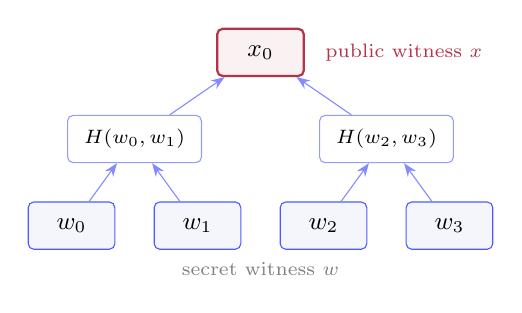
\begin{tikzpicture}[font=\small,
  n/.style={draw=accent,rounded corners=2pt,minimum width=11mm,minimum height=6mm,inner sep=1pt},
  sec/.style={n,fill=paper},
  mid/.style={n,draw=accent!60,minimum width=17mm,font=\scriptsize},
  pub/.style={n,draw=danger,thick,fill=danger!7},
  a/.style={-{Stealth},accent!70}]
\node[pub] (r) at (0,2.2) {$x_0$};
\node[mid] (h01) at (-1.6,1.1) {$H(w_0,w_1)$};
\node[mid] (h23) at ( 1.6,1.1) {$H(w_2,w_3)$};
\node[sec] (w0) at (-2.4,0) {$w_0$};
\node[sec] (w1) at (-0.8,0) {$w_1$};
\node[sec] (w2) at ( 0.8,0) {$w_2$};
\node[sec] (w3) at ( 2.4,0) {$w_3$};
\draw[a] (w0) -- (h01); \draw[a] (w1) -- (h01);
\draw[a] (w2) -- (h23); \draw[a] (w3) -- (h23);
\draw[a] (h01) -- (r); \draw[a] (h23) -- (r);
\node[font=\scriptsize,text=danger,anchor=west] at (0.7,2.2) {public witness $x$};
\node[font=\scriptsize,text=gray] at (0,-0.55) {secret witness $w$};
\end{tikzpicture}
\end{columns}
\pause

Note: we may use, e.g., $s, t, u, v, w$ instead of $w_0, \ldots, w_3$ or $x, y, z$ instead of $x_0, x_1, x_2$, as long as it's clear which are public and which are secret.
\end{frame}

\begin{frame}{Arithmetic Circuits and Constraints}
Arithmetic circuit: like a Boolean circuit, but
\begin{itemize}
\item wires carry values in $\mathbb F_p$.
\item gates are $+$ and $\cdot$.
\end{itemize}

\pause

Arithmetic circuits $\equiv$ systems of \emph{constraints}, one for each $+$ or $\cdot$ operation.

\end{frame}

\begin{frame}{Example: Constraint System and Witnesses}

A constraint system $C = \{C_0, C_1, C_2, C_3\}$:

$C_0: w_1 = w_0^2$\\
$C_1: w_2 = w_1^2$\\
$C_2: w_3 = w_2 + 5$\\
$C_3: w_3 = x_0$\\
\pause
\vspace{\baselineskip}
Here,
\begin{itemize}
\item $x = (x_0)$ is the public witness.
\item $w = (w_0)$ is the secret witness. \pause
\item $(w_1,w_2,w_3)$ are \emph{intermediate witnesses} (also secret). \pause
\item $\overline w = (w_0, w_1, w_2, w_3)$ is the \emph{extended} witness. \pause
\item $(\overline w, x) \vDash C$ means that all constraints hold.
\end{itemize}
\pause

In this case, $(w, x) \vDash C$ implies $x_0=w_0^4+5$. Conversely, when $x_0=w_0^4+5$ we can choose intermediate values satisfying $C$.
\end{frame}

\begin{frame}{A SNARK Only Proves the Encoded Relation}
\begin{center}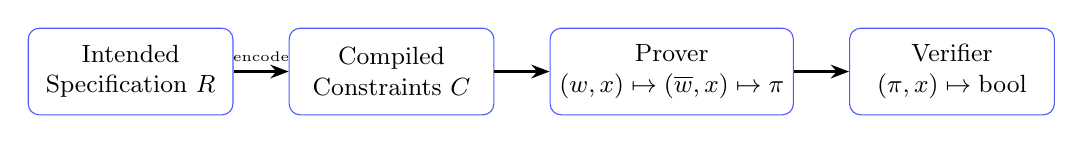
\begin{tikzpicture}[node distance=7mm, every node/.style={align=center,font=\small},b/.style={draw=accent,rounded corners,minimum width=26mm,minimum height=11mm}]
\node[b](spec){Intended\\Specification $R$};
\node[b,right=of spec](c){Compiled\\Constraints $C$};
\node[b,right=of c](proof){Prover\\$(w, x) \mapsto (\overline w, x) \mapsto \pi$};
\node[b,right=of proof](v){Verifier\\$(\pi, x) \mapsto \text{bool}$};
\draw[-{Stealth},thick](spec)--node[above,font=\tiny]{encode}(c);
\draw[-{Stealth},thick](c)--(proof);
\draw[-{Stealth},thick](proof)--(v);
\end{tikzpicture}\end{center}
\pause

Ideally:
\[\boxed{(\overline w, x) \vDash C \quad \Longleftrightarrow \quad R(w, x)}\]\vspace{-1mm}\begin{center}\footnotesize For a public-statement specification: $\exists w: (w, x) \vDash C \Leftrightarrow\exists w: R(w, x)$.\end{center}
\pause

An application can fail when one implication fails, even if the proof system works.
\end{frame}

\begin{frame}{Hints}
\begin{columns}[T]\column{.48\textwidth}
\textbf{Honest computation}
\[t \leftarrow w^2\]
The prover computes a \emph{hint} outside the circuit: if honest, with a witness generator.  The answer provided by the generator is called \emph{advice}.
\column{.48\textwidth}
\textbf{Enforced equation}
\[t-w^2=0\]
A constraint forces every accepted witness to respect that computation.
\end{columns}
\vspace{6mm}\begin{block}{The adversarial model}The prover may replace the witness generator, ignore advice, and substitute their own hints. Only the enforced constraints bind these choices.\end{block}
\note{4.25--5.5 minutes. A hint is not intrinsically unsafe. Explain that each hint needs enough constraints to establish the desired property, not necessarily a unique internal encoding.}
\end{frame}

%==============================================================
\section{Kinds of Underconstraint Bugs}
%==============================================================

\begin{frame}{Common Failure Patterns}
\begin{tabular}{>{\raggedright\arraybackslash}p{.30\textwidth}>{\raggedright\arraybackslash}p{.60\textwidth}}\toprule
Missing Requirement & What Can Go Wrong\\\midrule
Copy Constraint & Wires disconnect; values disagree.\\[2mm]
Range Check & Overflow or underflow; unexpected values.\\[2mm]
Hint Validation & Prover controls a computation.\\[2mm]
Field / Group Membership Check & Algebraic identities hold outside intended domain.\\[2mm]
Public Witness Binding & Malleability; i/o can be unrelated to circuit.\\\bottomrule\end{tabular}
\note{6.75--8 minutes. Mention disabled selectors and branch coverage. These patterns overlap. Use the table to connect the next examples.}
\end{frame}

\subsection{Missing Public Output Binding}

\titleslide{Example 0: Missing Public Output Binding}

\begin{frame}{Example: Missing Copy Constraint/Public Binding}
Suppose we omit $C_3: w_3 = x_0$ from our previous $C$.  
\pause

Let $C' = C \smallsetminus \{C_3\} = \{C_0, C_1, C_2\}$.

$C_0: w_1 = w_0^2$\\
$C_1: w_2 = w_1^2$\\
$C_2: w_3 = w_2 + 5$\\
\pause
\vspace{\baselineskip}

For every $x_0$, the prover can pick any $w_0$, compute $w_1, w_2, w_3$, and get $(\overline w, x) \vDash C'$.
\end{frame}

\begin{frame}{Example 0: Missing Binding $\to$ False Proof}
Claim: ``I know $w_0 \in \mathbb F_{11}$ such that $7 = w_0^4 + 5$'', i.e.\ $w_0^4 = 2$.
\pause

Fourth powers in $\mathbb F_{11}$:
\[\begin{array}{c|ccccccccccc}
w_0 & 0 & 1 & 2 & 3 & 4 & 5 & 6 & 7 & 8 & 9 & 10\\\hline
w_0^4 & 0 & 1 & 5 & 4 & 3 & 9 & 9 & 3 & 4 & 5 & 1
\end{array}\]
Note $R(w, 7)$ is false for every $w$.
\pause

But $\overline w = (1, 1, 1, 6)$ and $x_0 = 7$ satisfy $C'$:
\[1 = 1^2,\qquad 1 = 1^2,\qquad 6 = 1 + 5.\]
\pause
So the prover can produce a valid proof of a false claim.
\end{frame}

\begin{frame}{Repair: Public Input Binding}
Add a copy constraint to bind an intermediate witness to the public witness
\[C_3: x_0 = w_3.\]
\pause

Now $(w, x) \vDash \{C_0, C_1, C_2, C_3\} \Leftrightarrow R(w, x)$.
\pause

This copy constraint is the only link between what the circuit computes and what the verifier sees.
\end{frame}

\subsection{Unvalidated Hints}

\titleslide{Example 1: Unvalidated Hints}

\begin{frame}{Example 1: An Unvalidated IsZero Hint}
Let $w\in\F_{11}$ be a \textbf{secret witness} and $x\in\F_{11}$ a \textbf{public witness}.
\[R(w,x):\quad x=\operatorname{IsZero}(w)=\begin{cases}1&w=0,\\0&w\ne0.\end{cases}\]
\pause

Let $h$ be a secret hint. A witness generator advises
\[h=\begin{cases}w^{-1}&w\ne0,\\0&w=0.\end{cases}\]
\pause

Suppose the constraints are just
\[C_0:\qquad x=1-wh.\]
\pause
\textbf{Attack:} take $w=3$, $h=0$, $x=1$. Constraint $C_0$ holds, but $\operatorname{IsZero}(3) = 1$ is false.
\end{frame}

\begin{frame}{Repair: Constrain the Hint's Effect}
Add
\[\boxed{C_1:\ wx=0.}\]
If $w\neq 0$, the field property forces $x=0$, and $C_0$ then forces $h=w^{-1}$.

If $w=0$, $C_0$ forces $x=1$, and the value of $h$ does not matter.

A free hint is fine when it cannot reach the public output: witness non-uniqueness is not underconstraint.
\pause
\begin{block}{Lesson}
A hint need not have a unique representation (may have multiple valid $\overline w$ for a given $w$). The \emph{public behavior} must be pinned down by constraints.
\end{block}
\end{frame}

\subsection{Missing Boolean Check (Exercise)}

\titleslide{Exercise 2: A Selector}

\begin{frame}{Exercise 2: A Selector}
\textbf{Intended behavior:} $s$ selects $x$ or $y$.
\[s\in\{0,1\},\qquad z=\begin{cases}x&s=1,\\y&s=0.\end{cases}\]
\textbf{Implemented constraint over $\mathbb F_{11}$:}
\[\boxed{z=sx+(1-s)y}\]
Here $x, y$ are secret inputs.  Fix public output $z = 5$. The selector $s$ is secret.
\vspace{3mm}\begin{block}{Two minutes with your neighbour}
Suppose $x = 3, y = 7$.  Can you choose $s$ so that the equation accepts?\\ 
Which constraint is missing?
\end{block}
\end{frame}

\begin{frame}{Selector: False Witness and Repair}
\textbf{False Witness}

For $s=6$ in $\mathbb F_{11}$:
\[6\cdot3+(1-6)\cdot7=18-35=-17\equiv5\pmod{11}.\]
The implemented equation accepts, although $5\notin\{3,7\}$.
\pause

\textbf{Repair}
\[\boxed{s(s-1)=0}\qquad\text{and}\qquad z=sx+(1-s)y.\]
In a field, the new equation forces $s=0$ or $s=1$.
\end{frame}

\subsection{Range Checks and Foreign-Field Arithmetic}

\titleslide{Example 3: Range Checks and Foreign-Field Arithmetic}

\begin{frame}{A Boolean Check Is a 1-Bit Range Check}
$s(s-1) = 0 \Leftrightarrow s \in \{0, 1\}$: a range check on a single bit.
\pause

Field elements have no order and no sign. In $\mathbb F_{11}$, $3 - 5 = -2 = 9$.
\pause

So claims like ``balance $\geq$ withdrawal'' need a \emph{range check}: reading $x$ as an integer in $\{0, \ldots, p-1\}$, show $x < 2^n$.
\end{frame}

\begin{frame}{Range Checks by Bit Decomposition}
Claim: $x < 4$ in $\mathbb F_{11}$. Secret witnesses are the bits $w_0, w_1$:

$C_0: w_0(w_0 - 1) = 0$\\
$C_1: w_1(w_1 - 1) = 0$\\
$C_2: x = w_0 + 2w_1$\\
\pause

Then $x \in \{0, 1, 2, 3\}$, so $(w, x) \vDash C \Leftrightarrow R(x): x < 4$.
\pause

Pitfall: this needs $2^n \leq p$. With $4$ bits in $\mathbb F_{11}$, $x = w_0 + 2w_1 + 4w_2 + 8w_3$ and
\[3 = 1 + 2,\qquad 3 = 2 + 4 + 8 - 11.\]
Two bit patterns, $(1, 1, 0, 0)$ and $(0, 1, 1, 1)$, for the same $x$. If the circuit reads $w_3$ as ``$x \geq 8$'', the prover can claim $3 \geq 8$.
\end{frame}

\begin{frame}{Foreign-Field Arithmetic}
Sometimes a circuit over $\mathbb F_p$ must check arithmetic modulo some $\ell \neq p$ (e.g.\ elliptic-curve scalars). This is \emph{foreign-field arithmetic}.
\pause

Small example: native field $\mathbb F_{11}$, foreign modulus $\ell = 3$. Public $x, y, z \in \{0, 1, 2\}$ (already range-checked).

Define $R(x, y, z)$ if $xy \equiv z \pmod 3$.
\pause

Over the integers, $xy \equiv z \pmod 3 \Leftrightarrow xy - z = 3k$ for some quotient $k$. The prover supplies $k$ as a hint $w$:

$C_0: xy - z = 3w$

$C_1: w(w - 1) = 0$

\pause

Example: $x = y = 2$, $z = 1$: $4 - 1 = 3 \cdot 1$, so $w = 1$.
\end{frame}

\begin{frame}{Range-Check for Sound Modular Arithmetic}
$C_0: xy - z = 3w$ holds in $\mathbb F_{11}$, i.e.\ $xy - z - 3w$ is a multiple of $11$ as an integer.
\pause

With $x, y, z \in \{0, 1, 2\}$ and $w \in \{0, 1\}$:
\[xy - z - 3w \in \{-5, \ldots, 4\}.\]
\pause

The only multiple of $11$ in that range is $0$. So $xy - z = 3w$ holds over the integers, and $xy \equiv z \pmod 3$.
\pause

The range checks keep every term small enough that the native field never wraps.
\end{frame}

\begin{frame}{An Unbounded Quotient Checks Nothing}
Suppose we omit $C_1: w(w - 1) = 0$.
\pause

$3$ is invertible in $\mathbb F_{11}$ ($3^{-1} = 4$), so $C_0$ is satisfied by $w = (xy - z) \cdot 4$ for \emph{any} $x, y, z$.
\pause

False claim: $2 \cdot 2 \equiv 0 \pmod 3$. Take $w = (4 - 0) \cdot 4 = 16 = 5$:
\[3 \cdot 5 = 15 = 4 \text{ in } \mathbb F_{11}.\]
So $(w, x, y, z) = (5, 2, 2, 0) \vDash \{C_0\}$, but $R(2, 2, 0)$ is false.
\pause

Over the integers, $4 - 0 = 3 \cdot 5$ is false. The field wraps $15$ to $4$.
\pause

The quotient \emph{and} every other term must be range-checked, so that the native equation cannot wrap.
\end{frame}

\section{Deep Dive: gnark Fake GLV}
%==============================================================

\begin{frame}{Fake GLV: Checking a Hinted Scalar Multiplication}
\textbf{Goal}\quad Establish $Q=[s]P$ with fewer curve operations.
\vspace{3mm}
The prover supplies short scalars $u,v$ and the candidate point $Q$.
\[\underbrace{[u]P=[v]Q}_{\text{curve relation}},\qquad
\underbrace{u\equiv sv\pmod\ell}_{\text{scalar relation}}.\]
If $P,Q$ belong to a prime-order subgroup of order $\ell$ and $v\ne0\pmod\ell$, then
\[[v](Q-[s]P)=O\quad\Longrightarrow\quad Q=[s]P.\]
\textbf{Every hypothesis needs enforcement.}
\end{frame}

\begin{frame}{Two Fields Meet in One Gadget}
\begin{tabular}{lll}\toprule
Symbol & Meaning & Relevant arithmetic\\\midrule
$r$ & Native circuit field modulus & Coordinates in $\F_r$\\[2mm]
$\ell$ & Prime subgroup order & Scalars modulo $\ell$\\\bottomrule\end{tabular}\par
\vspace{5mm}
For BabyJubjub in a BN254 circuit, $r\ne\ell$.
\[u\equiv sv\pmod\ell\quad\text{is a relation in the scalar domain.}\]
An equation evaluated in $\F_r$ does not automatically enforce it.
\end{frame}

\begin{frame}{A Free Quotient Makes the Check Vacuous}
A simplified form of the vulnerable binding check:
\[\boxed{u-sv=k\ell\quad\text{in }\F_r}\]
Here $k$ is a prover-supplied field element without sufficient bounds.
Since $\ell\ne0$ in $\F_r$,
\[k=(u-sv)\ell^{-1}\pmod r\]
exists for \emph{every} choice of $u,s,v$.
\vspace{3mm}The equation constrains $k$. It imposes no binding between $u$, $s$, and $v$.
\end{frame}

\begin{frame}[fragile]{The gnark Assertion Behind the Algebra}
\begin{lstlisting}[language=Go,basicstyle=\ttfamily\footnotesize]
// Excerpt from the supplied v0.15.0 case study
s, _ := api.NewHint(halfGCD, 4, checkedScalar, curve.Order)
s1, s2, bit, k := s[0], s[1], s[2], s[3]
vs := api.Mul(s2, checkedScalar)
kL := api.Mul(k, curve.Order)
lhs := api.Select(bit, s1, api.Add(s1, vs))
rhs := api.Select(bit, api.Add(kL, vs), kL)
api.AssertIsEqual(lhs, rhs)
\end{lstlisting}
For a Boolean sign bit, the branches assert $u-sv=k\ell$ or $u+sv=k\ell$ in $\F_r$.
\vspace{2mm}Both branches let the free quotient absorb the discrepancy. Bounds on $s_1,s_2$ do not bind $k$.
\src{https://github.com/Consensys/gnark/pull/1765}{Source excerpt: supplied HTML case study. PR \#1765 is its cited repair.}
\end{frame}

\begin{frame}{What a False Scalar Multiplication Means}
Choose $u=0$, $v=1$, and $Q=O$.
\[[u]P=[v]Q=O.\]
The free quotient satisfies the native-field equation for any $s$.
Thus the gadget can accept $Q=O$ even when $[s]P\ne O$.
\par\vspace{4mm}\textbf{Signature verification context}
\[[S]B=R+[h]A,\qquad h=H(R,A,m).\]
If the gadget replaces $[h]A$ by $O$, the equation loses its intended key and message binding.
\end{frame}

\begin{frame}{Fake GLV Repair: Restore Every Hypothesis}
To infer $Q=[s]P$ from $[u]P=[v]Q$, require:
\begin{enumerate}
\item A \textbf{sound scalar congruence} $u\equiv sv\pmod\ell$ (proper foreign-field arithmetic or equivalent sound encoding).
\item $P,Q$ in the intended \textbf{prime-order subgroup} of order $\ell$.
\item $v\not\equiv0\pmod\ell$, so multiplication by $v$ is invertible on that subgroup.
\item Sound constraints on signs, decomposition bounds, and the selected branches.
\end{enumerate}
\vspace{1mm}
Then $[v](Q-[s]P)=O$ and cancellation gives $Q=[s]P$.
\begin{block}{Crucial point}Bounding the quotient $k$ \emph{alone} does not establish the foreign-field relation. All terms need sound bounds/carry reasoning so native-field wraparound cannot invalidate the integer argument.\end{block}
\src{https://github.com/Consensys/gnark/pull/1765}{gnark PR \#1765 (verify precise affected paths and releases before attribution).}
\end{frame}

%==============================================================
\section{Finding Underconstraints}
%==============================================================

\subsection{Manual Review}

\begin{frame}{Manual Review Starts From the Specification}
\begin{enumerate}
\item Write the intended domain and input/output relation.
\item Mark every public witness, secret witness, hint, and selector.
\item Trace the constraints that bind each required property.
\item Try a value outside the intended domain.
\item Add the missing constraint and retain the counterexample as a regression.
\end{enumerate}
\vspace{3mm}For the selector, the equation covered interpolation. The specification also required a Boolean domain.
\end{frame}

\begin{frame}{Honest-Witness Tests Leave a Gap}
\textbf{Typical positive test}
\[\overline w\leftarrow\operatorname{HonestWitness}(x),\qquad (\overline w, x) \vDash C.\]
\textbf{Soundness question}
\[\exists \overline w, x:\ C(\overline w, x)=0\ \land\ \neg R(w, x)\ ?\]
\begin{itemize}
\item Positive tests check examples of valid executions.
\item Adversarial witness tests search outside the honest generator's outputs.
\item Missing constraints can leave every positive test passing.
\end{itemize}
\end{frame}

\subsection{Fuzzing}

\begin{frame}{Random Search versus Structured Witnesses}
Randomly changing only public inputs often runs the honest witness generator and misses underconstraints.
\vspace{3mm}

\textbf{Mutate private witnesses and hints:} change a selector, quotient, or candidate point while keeping other constraints satisfiable.
\vspace{3mm}

\textbf{Structured attacks beat blind random search:} if a quotient $k$ is free, calculate $k=(u-sv)\ell^{-1}$ directly rather than guessing it.
\end{frame}

\begin{frame}[fragile]{Demo: Fuzz the Relation, Including the Witness}
\begin{lstlisting}[language=Python]
# F_11; bypass the honest selector generator
x, y = 3, 7
for _ in range(1000):
    b = rng.randrange(11)
    z = (b*x + (1-b)*y) % 11
    if accepts(x, y, z, b) and z not in (x, y):
        report_counterexample(x, y, z, b)
        break
\end{lstlisting}
\textbf{Oracle:} acceptance plus a violation of the independent specification.\\[2mm]
Randomize hints and private wires. Preserve the constraints you want to test.
\end{frame}

\subsection{Formal Verification}
\begin{frame}{Formal Verification: Search for an Invalid Witness}
For public witness $x$ and extended secret witness $w$, check satisfiability of
\[\boxed{\exists w, x:\ C(w, x)=0\ \land\ \neg R(w, x).}\]
\begin{itemize}
\item \textbf{SAT:} a witness-level counterexample to the specification exists.
\item \textbf{UNSAT:} no counterexample exists \emph{in the encoded model}.
\item \textbf{UNKNOWN / timeout:} no verification conclusion.
\end{itemize}
\vspace{1mm}
For the selector: $z=sx+(1-s)y$ and $z\notin\{x,y\}$ is satisfiable. 
\pause

Add $s(s-1)=0$: the query becomes unsatisfiable over every field.
\end{frame}

\section{Verification Infrastructure and AI}
% Insert these two frames into the existing Beamer document.
% Requires: \usepackage{tikz} and \usetikzlibrary{positioning,arrows.meta,calc}
% Uses existing deck colors: accent, paper, ink, danger.

\begin{frame}[shrink=12]{Formal Verification: Toward a Unified Framework}
\centering
\vspace*{7mm}
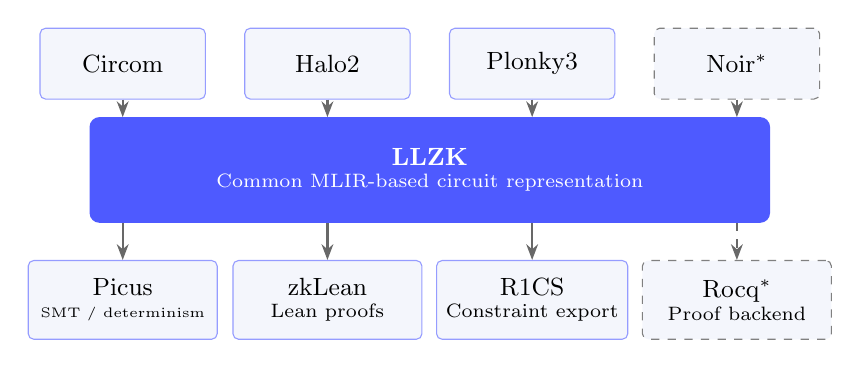
\begin{tikzpicture}[>=Stealth, font=\small,
  frontend/.style={draw=accent!60, rounded corners=2pt, fill=paper, minimum width=21mm,minimum height=9mm,align=center},
  backend/.style={draw=accent!60, rounded corners=2pt,fill=paper,minimum width=24mm,minimum height=10mm,align=center},
  arrow/.style={-{Stealth[length=2mm]},line width=.8pt,draw=ink!65}]
  \node[frontend] (circom) at (-3.9,2.1) {Circom};
  \node[frontend] (halo) at (-1.3,2.1) {Halo2};
  \node[frontend] (plonky) at (1.3,2.1) {Plonky3};
  \node[frontend,dashed,draw=gray] (noir) at (3.9,2.1) {Noir$^{*}$};
  \node[draw=accent,rounded corners=3pt,very thick,fill=accent,text=white,minimum width=86mm,minimum height=13mm,align=center] (llzk) at (0,.75) {\textbf{LLZK}\\[-1mm]{\scriptsize Common MLIR-based circuit representation}};
  \node[backend] (picus) at (-3.9,-.9) {Picus\\[-1mm]{\tiny SMT / determinism}};
  \node[backend] (lean) at (-1.3,-.9) {zkLean\\[-1mm]{\scriptsize Lean proofs}};
  \node[backend] (r1cs) at (1.3,-.9) {R1CS\\[-1mm]{\scriptsize Constraint export}};
  \node[backend,dashed,draw=gray] (rocq) at (3.9,-.9) {Rocq$^{*}$\\[-1mm]{\scriptsize Proof backend}};
  \foreach \a in {circom,halo,plonky}{\draw[arrow] (\a.south) -- (\a.south |- llzk.north);}
  \draw[arrow,dashed] (noir.south) -- (noir.south |- llzk.north);
  \foreach \b in {picus,lean,r1cs}{\draw[arrow] (llzk.south -| \b.north) -- (\b.north);}
  \draw[arrow,dashed] (llzk.south -| rocq.north) -- (rocq.north);
\end{tikzpicture}
\vspace{1mm}
\begin{block}{Why it matters}
One intermediate representation enables reusable analyses across circuit languages; \emph{LLZK is infrastructure, not itself a soundness proof}.
\end{block}
{\setlength{\parskip}{0pt}\tiny $^{*}$Evolving integrations / research directions, not universal production support.\par LLZK is open source, developed by Veridise with support from the Ethereum Foundation. \url{https://github.com/project-llzk}\par
\color{gray}\textbf{Scalability note:} Bit-blasting large-prime-field arithmetic into Boolean constraints can be costly. Generic SMT solvers may struggle with nonlinear field operations; specialized algebraic reasoning and circuit-aware verification backends help. LLZK provides the representation, not the solver.\par}
\end{frame}

\begin{frame}{Why AI-Assisted Review? The Dependency Problem}
\begin{columns}[T,onlytextwidth]
\column{.47\textwidth}
\centering
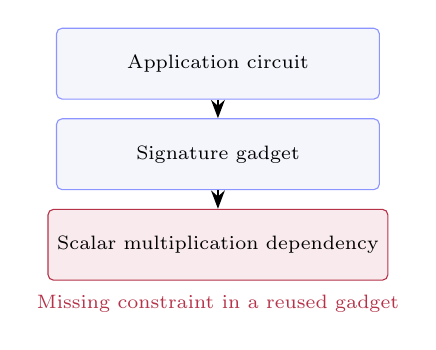
\begin{tikzpicture}[>=Stealth,font=\scriptsize,
  n/.style={draw=accent!65,rounded corners=2pt,fill=paper,minimum width=41mm,minimum height=9mm,align=center},
  risk/.style={draw=danger,fill=danger!10,rounded corners=2pt,minimum width=41mm,minimum height=9mm,align=center}]
  \node[n] (app) at (0,1.6) {Application circuit};
  \node[n] (sig) at (0,.45) {Signature gadget};
  \node[risk] (mul) at (0,-.7) {Scalar multiplication\ dependency};
  \draw[-Stealth,thick] (app)--(sig);
  \draw[-Stealth,thick] (sig)--(mul);
  \node[align=center,text=danger] at (0,-1.45) {Missing constraint in a reused gadget};
\end{tikzpicture}
\column{.53\textwidth}
\textbf{Why manual review alone is hard}
\begin{itemize}\setlength{\itemsep}{1mm}
\item Security assumptions cross library and compiler boundaries.
\item Advisories, versions, and reachable call paths change.
\item Honest-witness tests can pass even when a dependency is underconstrained.
\end{itemize}
\end{columns}
\vspace{2mm}
\begin{block}{AI-assisted workflow}
\textbf{Find} relevant advisories $\to$ \textbf{trace} affected call paths $\to$ \textbf{propose} malicious witnesses $\to$ \textbf{verify} using tests, solvers, or proofs.
\end{block}
\centering\small\textbf{AI broadens the search; executable evidence establishes the finding.}
\end{frame}

\begin{frame}{How We Review ZK Systems at OpenZeppelin}
\small
\begin{center}
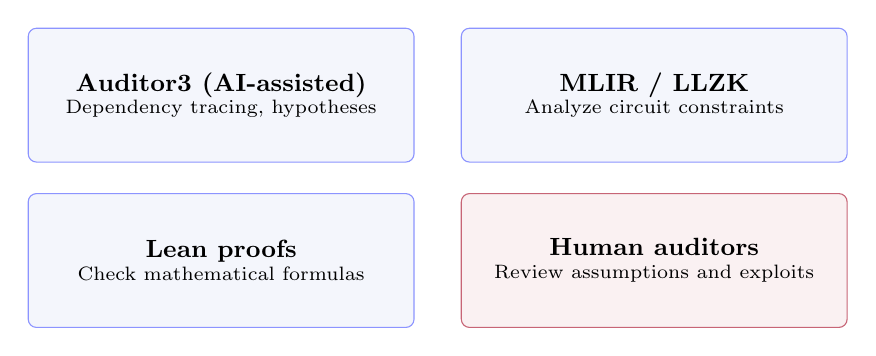
\begin{tikzpicture}[font=\small,
  tool/.style={draw=accent!65,rounded corners=3pt,fill=paper,
  minimum width=49mm,minimum height=17mm,align=center,inner sep=3pt},
  human/.style={draw=danger!75,rounded corners=3pt,fill=danger!7,
  minimum width=49mm,minimum height=17mm,align=center,inner sep=3pt}]
  \node[tool] (ai) at (-2.75,1.15) {\textbf{Auditor3 (AI-assisted)}\\[-1mm]{\scriptsize Dependency tracing, hypotheses}};
  \node[tool] (mlir) at (2.75,1.15) {\textbf{MLIR / LLZK}\\[-1mm]{\scriptsize Analyze circuit constraints}};
  \node[tool] (lean) at (-2.75,-.95) {\textbf{Lean proofs}\\[-1mm]{\scriptsize Check mathematical formulas}};
  \node[human] (people) at (2.75,-.95) {\textbf{Human auditors}\\[-1mm]{\scriptsize Review assumptions and exploits}};
\end{tikzpicture}
\end{center}
\vspace{2mm}
\begin{block}{Complementary approaches}
AI helps find places to look; formal methods establish selected properties; human reviewers connect the proofs and counterexamples to the real security model.
\end{block}
\centering {\footnotesize \textbf{None alone establishes end-to-end security.}}
\end{frame}

\section{Wrap-Up}
%==============================================================



\begin{frame}[fragile]{Questions}
\begin{columns}[c]
\column{.66\textwidth}
{\Large Which property does your circuit need to enforce?\par}
\vspace{5mm}
\textbf{Run the counterexamples yourself}
\begin{lstlisting}[basicstyle=\ttfamily\scriptsize]
git clone https://github.com/V-k-h/training-for-constraining
cd training-for-constraining
make demo   # five counterexamples over F_11
make test   # exhaustive checks of the repairs
make lean   # optional: machine-checked theorems
\end{lstlisting}
{\footnotesize Python 3.10+ only. Lean 4 and LLZK material is optional.\par}
\column{.30\textwidth}
\centering
\qrcode[height=34mm]{\repourl}\\[2mm]
{\scriptsize\url{\repourl}}
\end{columns}
\end{frame}

\appendix
\begin{frame}{Appendix: Source Reports}
\small\begin{itemize}
\item \href{https://shieldedlabs.net/the-orchard-counterfeiting-vulnerability/}{Shielded Labs: Orchard counterfeiting disclosure (June 4, 2026)}.
\item \href{https://nvd.nist.gov/vuln/detail/CVE-2026-54496}{Orchard missing-copy-constraint technical description}.
\item \href{https://github.com/openvm-org/openvm/security/advisories/GHSA-76mq-v757-53gr}{OpenVM: CVE-2026-46669 (May 15, 2026)}.
\item \href{https://forum.scroll.io/t/report-scroll-mainnet-emergency-upgrade-on-2026-02-23/1412}{Scroll Security Council: February 23 emergency upgrade report}.
\item \href{https://veridise.com/wp-content/uploads/2026/05/VAR_zksync_260216_picus_fuzzing-_Veridise_Security_Audit_AuditHub.pdf}{Veridise: Airbender tooling report (April 22, 2026), pp. 3, 11--17}.
\end{itemize}
\end{frame}

\begin{frame}{Appendix: Fake GLV and Further Reading}
\small\begin{itemize}
\item Supplied reference: \texttt{fake-glv-underconstraint.html}. Main workshop uses its algebraic example, with explicit subgroup assumptions.
\item \href{https://github.com/Consensys/gnark/pull/1765}{gnark PR \#1765: repair cited by the supplied reference}.
\item \href{https://ethresear.ch/t/fake-glv-you-dont-need-an-efficient-endomorphism-to-implement-glv-like-scalar-multiplication-in-snark-circuits/20394}{Fake GLV: original method discussion (2024)}.
\item \href{https://blog.zksecurity.xyz/posts/openvm-bugs/}{ZKSecurity: AI-assisted OpenVM discovery (2026)}.
\end{itemize}
\vspace{4mm}The fake-GLV production version and patch claims come from the supplied reference. Check the release advisory before presenting exact affected-version ranges.
\end{frame}

\begin{frame}{Appendix: A Source-Linked Dependency Review Inventory}
\small\begin{tabular}{>{\raggedright\arraybackslash}p{.24\textwidth}>{\raggedright\arraybackslash}p{.64\textwidth}}\toprule
Published example & Review question\\\midrule
\href{https://github.com/Consensys/gnark/security/advisories/GHSA-95v9-hv42-pwrj}{gnark signature malleability} & Does the caller establish the required scalar range?\\[2mm]
\href{https://github.com/Consensys/gnark/security/advisories/GHSA-rjjm-x32p-m3f7}{gnark range-check width} & Does the enforced bound match the application's intended width?\\[2mm]
\href{https://github.com/Consensys/gnark/security/advisories/GHSA-9fvj-xqr2-xwg8}{gnark fake-GLV DoS} & Can hostile inputs make witness generation stall? This is distinct from our soundness case.\\[2mm]
\href{https://github.com/openvm-org/openvm/security/advisories/GHSA-76mq-v757-53gr}{OpenVM pairing soundness} & Does the optimized check enforce the required subfield?\\\bottomrule\end{tabular}\par
\vspace{3mm}Illustrative inventory, not a complete issue list. Applicability requires version and call-path review.
\end{frame}

\begin{frame}{Appendix: Why Short Scalars Help}
\[u\equiv sv\pmod\ell,\qquad |u|,|v|\text{ roughly }\sqrt\ell.\]
The honest prover finds a short lattice vector, often with an extended-Euclidean or half-GCD method.
\begin{itemize}
\item Short scalars reduce the double-and-add work in $[u]P-[v]Q$.
\item Finding the decomposition happens outside the circuit.
\item The circuit still needs to enforce its algebraic relation, signs, bounds, and nonzero denominator.
\end{itemize}
\end{frame}
\end{document}
